\documentclass[a4paper,12pt]{report}

\usepackage{alltt, fancyvrb, url}
\usepackage{graphicx}
\usepackage{subfigure}
\usepackage{wrapfig}
\usepackage{float}
%\usepackage{algorithmic}
\usepackage[utf8]{inputenc}
\usepackage{fontenc}
\usepackage{amsthm}
\usepackage[english]{babel}
%stmaryrd,algorithm
\usepackage{amsmath,mathtools}
\usepackage{amssymb}
% Remove option to use English naming
\usepackage[english]{cleveref}
\graphicspath{ {img/} }

\title{Supervised Project ``Bicriteria Paths Problem''}
 
\author{Andrea Rossolini}
\date{\today}


\begin{document}
 
\maketitle

\begin{abstract}
In this paper I analyze a \textit{pathfinding} problem starting from a classical shortest path problem and then, after several optimization, going to resolve a graph that utilizes two static weights on his arches, considering the most full satisfying set of solutions.

As is known, Dijkstra's algorithm is most widely used to solve routing problems; in fact is very easy to create an implementation that attempts to find the best path in a classical weighted graph. So I will focus on the operations of optimization.
%
The most important part of the paper is the one that analyze the paths of a graph with two weights for each arches of it, one value represent the distance (also present in the monocriteria problem) and the other represent the danger of that arch. So the implementation will find not only the shortest and safest path, but also all the paths (not dominated) that take intermediate values. Two different algorithms will be shown for the analysis of the bicriteria problem.
\end{abstract}

\tableofcontents

\chapter{Introduction}
Dijkstra's algorithm, as already mentioned above, is widely used to find shortest path in routing problems that's use graphs with not-negative, static values. But this algorithm takes into consideration only one "dimension" of costs; for example, to calculate a path from the source node to the destination, distance is the result of adding up the length between two nodes segment by segment.
%
But the problem faced in our study considers two criteria for choosing the wanted path: the first cost defines the distance, while the second one represent the danger. So, the problem with Dijkstra is that we will found a path very short, but very dangerous, or vice versa. Concerning multicriteria shortest path problem is intended to determine a path that optimizes the costs from a source to the target, but, in general, there is no a single optimal solution, so the goal of this project is to determinate a set of feasible and not-dominated solution, founding different paths 
based on the two criteria, so is not sufficient minimizing distance or danger, but the relations between this two values.
\vspace{5mm}

\begin{figure}
	\centering
	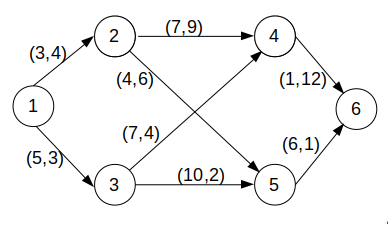
\includegraphics[width=\linewidth]{img/exampleGraph1}
	\caption{Graph example.}
	\label{fig:graphExample}
\end{figure}

\begin{table}[]
	\centering
	\begin{tabular}{|c|c|c|}
		\hline
		$p1$ & $1\to2\to4\to6$ & (11, 25) \\ \hline
		$p2$ & $1\to2\to5\to6$ & (13, 11)  \\ \hline
		$p3$ & $1\to3\to5\to6$ & (21, 6)  \\ \hline
		$p4$ & $1\to3\to4\to6$ & (13, 18)  \\ \hline
	\end{tabular}
	\caption{Graph's solution}
	\label{tab:graphExample}
\end{table}

In fig.\ref{fig:graphExample} is shown an example of a double criterion's routing. The nodes are labeled with numbers $\{1,2, ..., 6\}$ and the weights of the arches are represented as a pair of value (\textit{a, b}), where \textit{a} is distance and \textit{b} is danger.

In table \ref{tab:graphExample} are shown all the possible graph's iterations, $p1$ and $p3$ respectively the shortest and the safest paths, $p2$ is a not-dominated solution (it is longer than $p1$ but safer, more dangerous then $p3$, but, in this case, shorter) and $p4$ is a dominated path, so is useless to us.


 
\section{Mathematical formulation}

Let $G(N,A)$ denotes direct network which is composed of a finite set $N=\{0,1, \dots, n\}$ of nodes and a finite set $A \subseteq N\times N $, that represents the set of directed edges. Each arc can be denoted as an order pair $(i,j)$, where $i\in N$, $j \in N$ and both are two different nodes in $G(N,A)$.\\
Let define $c^k_{i,j}$ where $(i,j)\in A$ and $1\leq k \leq 2$ (because we are talking about a double criterion problem) represent the cost which we are referring to. We define two nodes in the graph: $s$ and $t$, where $s \in N$ and $t \in N$, these are respectively the \textit{source} and \textit{target} of which we want to find one or more paths.
%dei quali noi vogliamo trovare uno o più percorsi
We can qualify a path $p_{s,t}$ as a sequence  of  alternating nodes and arcs $p_{s,t} = \{s, (s, i_1), i_1, \dots, i_{l}, (i_l,t), t\}$.\\
So we said that each $c^k_{i,j}$ refers to one of the two costs of each arch $(i,j)$, therefore the total cost of the entire path can be represented in this way:\\

\begin{gather}(c^1(p_{s,t}), c^2(p_{s,t}))\end{gather}
\begin{gather}c^1(p_{s,t})=\sum_{(i,j)\in p}c^1_{i,j}\end{gather}
\begin{gather}c^2(p_{s,t})=\sum_{(i,j)\in p}c^2_{i,j}\end{gather}
Our purpose is to \textbf{minimize} the $(1.2)$ to find the shortest path or the $(1.3)$ to find the safest one.

\chapter{Mono-criteria algorithms}

In this chapter will be explained the algorithms which concern the single criteria routing.
The analysis focuses on the evolution and optimization of the following algorithm, explaining some implementation choices.

\section{Dijkstra's algorithms}

Dijkstra's algorithm is a very famous algorithm used to find the shortest paths between nodes in a graph connected by arches with positive weights.\\
Different implementation of this algorithm are present in this paper, as follows are all explained.

\begin{figure}[h]
	\centering
	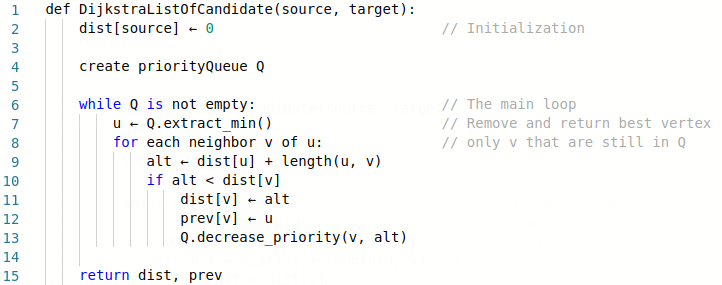
\includegraphics[width=\linewidth]{img/dijkstraLoC.png}
	\caption{Pseudocode - Dijkstra (List of Candidates)}
	\label{fig:dijkstraLoC}
\end{figure}

\subsection{One to all}
This implementation is useful to find \textbf{all the shortest path} from a source node to each other graph's nodes. The starting node will save a dictionary where there is a key for each reached node and the respective value of distance.
It implement a \textit{priority queue} so the complexity of this implementation is $O((|N|+|A|)\log_2(|N|))$ where $N$ is the number of vertices and $A$ the number of edges. In the worst case, so where $A>>N$, the time complexity is $(|A|\log_2(|N|))$.

This implementation explores all the nodes reachable from the source; so it doesn't stop until the graph is totally explored.

\subsection{One to one}
This implementation focuses to find the shortest path between the node source and the target, using the classical implementation of Dijkstra's algorithm.\\
The difference from this to the previous implementation is that this doesn't use a priority queue, but the algorithm will interrogate each not-visited node every loop; this is very time consuming, in fact the complexity of this implementation is $O(|N^2|)$.
%TODO: controlla la grammatica qua
%la differenza tra questa e la precedente implementazione sta nel fatto che questa non implementa 

\subsection{List of candidate}
The last version of Dijkstra's algorithm is an implementation that uses a priority queue. The elements of this queue are insert by each new visited node, so the queue's elements are the neighbors of the visited node; in this way the algorithm needs to interrogate only some nodes and not all graphs.\\
The list of candidate algorithm has the same \textit{worst-case complexity} of the \textit{One to all} algorithm: $O((|N|+|A|)\log_2(|N|))$.

This implementation is faster than the previous: details of improvement are visualized and studied in the dedicated section.

\section{''A Star'' algorithm}
The A Star algorithm (or 'A*') is almost an extension of Dijkstra's algorithm, but it achieves better performance and accuracy by using (generically) heuristics. To determinate which of its paths to extend, A* does so based on the cost of the path and an estimate of the cost required to expand the path to the goal.

So A* select nodes that minimize:
$$ f(n) = g(n) + h(n)$$
\begin{itemize}
	\item $n$ is the next path's node
	\item $g(n)$ is path's cost from the beginning to $n$
	\item $h(n)$ is the heuristic function
\end{itemize}
Heuristic, in this case, is the shortest distance from $n$ to the goal, so a \textit{straight-line} or better the \textbf{euclidean distance} to the target.
According with \footnote{\url{https://en.wikipedia.org/wiki/A*_search_algorithm}} the time complexity is related to $h$ and the number of nodes explored is exponential in the depth of the shortest path solution.
So the worst case is $O(|N|) \equiv O(b^d)$ where $b$ is the average number of successors per node and $d$ the depth of the solution.
\subsubsection*{implementation's details}
At each iteration:
\begin{enumerate}
	\item The node with the lowest $f(x)$ is popped by the queue (implemented as a priority queue).
	\item Update the values of the neighbors and then add them to the queue.
	\item The algorithm repeat until the goal is visited.
\end{enumerate}
The Euclidean distance between two points is: $$\sqrt{(i_x - t_x)^2 + (i_y - t_y)^2}$$
where $i$ is a node of the graph and $t$ the target, $x$ and $y$ are latitude and longitude.


\section{Analysis of the results}
This paragraph shows the principal characteristics and results of each implementation.
\subsection{Time consuming} 
In the figure \ref{fig:monoCriteriaOutput} are shown some results, from 15 different iteration, classified in three "set" that groups different path's length.
\begin{figure}[H]
	\centering
	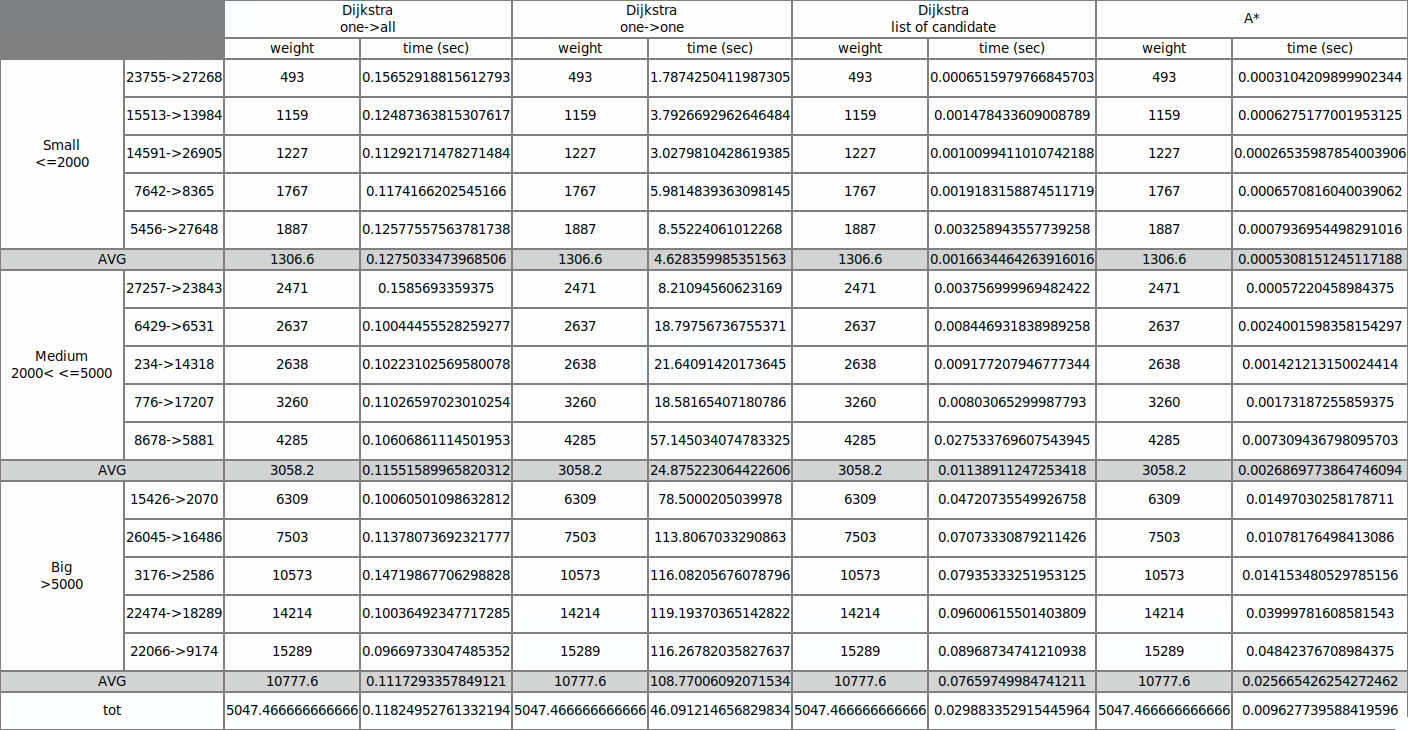
\includegraphics[width=\linewidth]{monoCriteriaOutput.png}
	\caption{Performance of the mono-criteria algorithms}
	\label{fig:monoCriteriaOutput}
\end{figure}
As possible to get from the table, we can recognize that the first column, '\textit{one$\to$all}', has a pretty much constant elaboration time (it comprehends the algorithm's work completion and the research in target node's attribute the distance from source). From the data of \textit{one$\to$one} algorithm is easily to recognize that the implementation without a priority queue is unsustainably slow, especially in the longest paths. From the latest two algorithm is possible to see that the \textit{A Star}'s implementation is more the 3 times faster than the \textit{List of candidate}, than from his part is near to be ten times more performing than the one to all implementation (which uses a priority queue).

\subsection{Node visited}

All the implementation are going to find the same paths between nodes; in particular all the implementation (except for the \textit{A Star}'s algorithm) explore the same nodes, instead, the 'not-Dijkstra's algorithm', explores less number of nodes, this means that it makes less loops during the elaboration and research of the shortest path.

In the following images is shown how, researching the shortest path, the algorithms visit nodes in a different way:\\
Dijkstra's algorithm (\textit{list of candidate}) makes a research more "circling" around the source (big green point), instead the 'A Star', for his nature, is more direct and it reaches the target exploring an "oval" between the starting nodes and the target. So is easy to see and understand how the last implementation is more efficient than the others.  
%TODO: add images of paths

\chapter{Bicriteria algorithms}

In this chapter are explained the algorithms implemented to studying the case of a graph with arches having two different weights.
Keeping in mind the mathematical explanation made in the introduction, we can enunciate some definitions:

\theoremstyle{definition}
\newtheorem{definition}{Definition}
\begin{definition}{Feasible solution}\\
	Let $x, y$ be two distinct feasible path from a source $s$ to a target $t$. We say $x$ \emph{dominates} $y$ if and only of $c^k(x) \leq c^k(y)$ $\forall$ $k \in [1,2]$.
\end{definition}

\theoremstyle{definition}
\begin{definition}{Pareto front}\\
	For a given set of feasible solutions there is a subset of optimal solutions. It is simpler to understand graphically.
\end{definition}

\section{Dijkstra applied to bicriteria}
So, by the fact that we have to deal with two criterion, it's possible to introduce another variable: $\alpha$.\\
We also can now set the following variables: the distance $dist=c^1$ and the danger $dang=c^2$.\\
According with the function: 
\begin{equation}\label{eq:pareto front}
	\alpha*dist + (1-\alpha) dang = k
\end{equation}
\begin{center}
	where $k$ is constant and $\alpha \in [0, 1]$.
\end{center}
We can say that our graph $G=(N,V,dist,dang)$ is reducible to $G=(N,V,\alpha*dist + (1-\alpha) dang)$ and we can address the problem as the previous case, so using Dijkstra's algorithm (list of candidates) giving a value to $\alpha$.\\
It is easy to deduce that plus the value of $\alpha$ approaches $0$ means to find safest paths, instead, more $\alpha$ is near to $1$ means that we'll found shortest paths.

\vspace{5mm}

The algorithm's implementation is similar to Dijkstra's list of candidate, but with the difference that this version needs in input, as well as the source and the target, the value of $\alpha$; then, using \eqref{eq:pareto front}, the algorithm will choose the optimal path.

\begin{figure}[h]
	\centering
	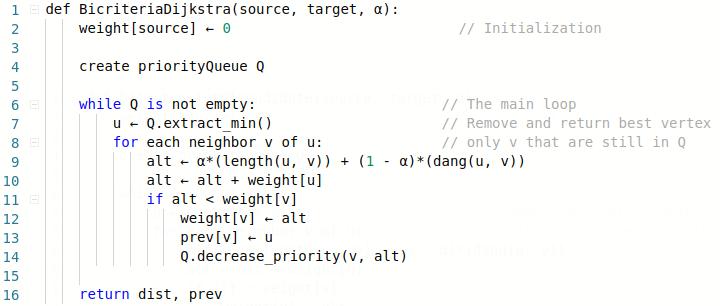
\includegraphics[width=\linewidth]{img/bicriteriaDijkstra.png}
	\caption{Pseudocode - Dijkstra with two criterion}
	\label{fig:bicriteriaDijkstra}
\end{figure}
\
\subsection{Application of Bicrtieria Dijkstra}
The aforementioned algorithm is able to identify the most of the solution 
To use aforementioned algorithm, have been implemented two different functions.

\subsubsection{Bicriteria Dijkstra iteration}
This is a very raw version, its operation is based on recalling the pathfinding function, a lot of time, but every time with a different value for $\alpha$.

It is very time consuming, because it has to call the same function a lot of time and probably with the same result, and its precision is related to the increasing value for $\alpha$.

\subsubsection{Bicriteria Dijkstra with binary research}
This version is an "evolution" of the last one, because it uses \textit{binary research}. It is based on calling the function at least two time: with $\alpha = 0$ and $\alpha=1$, then, if the result is different, with $\alpha=0.5$, again, if the result is different with $\alpha=\alpha/2$, and so on and so on; until there's no more solution.

This version is more efficient and precise than the other one.

%TODO: make a little proof of this

% \subsection*{Esempio di buona suddivisione in package}
% L'applicazione è stata divisa in tre sottoparti logiche, come descritto nell'architettura: Model, Controller e Boundary. Maggiori dettagli sulle scelte fatte:
% \begin{itemize}
%  \item Radice: non avendo alcun dominio, abbiamo deciso di utilizzare il prefisso dell'Università, cui abbiamo aggiunto un nostro identificativo: \texttt{it.unibo.studentsgroup}. Inoltre, abbiamo aggiunto un suffisso che indentifica questo progetto, per cui tutti i package saranno prefissi da: \texttt{it.unibo.studentsgroup.thisapp}.
%  \item Abbiamo diviso l'applicazione in tre sottoparti logiche in architettura, la divisione in package le rispecchia: \texttt{.model}, \texttt{.control}, \texttt{.boundary}. 
%  \item Essendo la parte di gestione dell'I/O composta di molti sorgenti, abbiamo suddiviso \texttt{.boundary} in sottopackage: \texttt{.boundary.network} e \texttt{.boundary.local}.
%  \item All'interno del model il concetto di \texttt{InterfacciaMoltoUsata} è stato implementato da numerose classi diverse. Di conseguenza, abbiamo adottato un subpackage \texttt{.model.imoltousata} dove abbiamo organizzato tutte le implementazioni, rendendo più navigable il package \texttt{it.unibo.studentsgroup.thisapp.model}.
% \end{itemize}


\subsection*{Esempi di UML ben realizzati}

In questa sezione ci si concentrerà sugli aspetti di personalità e sul funzionamento del reporting di GLaDOS.

Il sistema per la gestione della personalità utilizza il pattern Strategy, come da \Cref{img:strategy}: le implementazioni di Personality possono essere modificate, e la modifica impatta direttamente sul comportamento di GLaDOS.


Sono state attualmente implementate due personalità, una buona ed una cattiva.
Quella buona restituisce sempre una torta valida, mentre quella cattiva restituisce sempre una torta.
Dato che le due personalità differiscono solo per il comportamento da effettuarsi in caso di percorso completato con successo, è stato utilizzato il pattern template method per massimizzare il riuso, come da \Cref{img:template}.
Il metodo template è onSuccess(), che chiama un metodo astratto e protetto makeCake().



\subsection*{Elementi positivi}

\begin{itemize}
 \item Si descrivono molto brevemente i componenti che si è deciso di sottoporre a test automatizzato.
 \item Si utilizzano suite specifiche (e.g. JUnit) per il testing automatico.
 \item Se sono stati eseguiti test manuali di rilievo, si elencano descrivendo brevemente la ragione per cui non sono stati automatizzati. Ad esempio, se tutto il team sviluppa e testa su uno stesso sistema operativo e si sono svolti test manuali per verificare, ad esempio, il corretto funzionamento dell'interfaccia grafica o di librerie native su altri sistemi operativi, può avere senso menzionare la cosa.
\end{itemize}

\subsection*{Elementi negativi}
\begin{itemize}
 \item Non si realizza alcun test automatico.
 \item La non presenza di testing viene aggravata dall'adduzione di motivazioni non valide.
 \item Si descrive un testing di tipo manuale in maniera prolissa.
 \item Si descrivono test effettuati manualmente che sarebbero potuti essere automatizzati, ad esempio scrivendo che si è usata l'applicazione manualmente.
\end{itemize}

\section{Metodologia di lavoro}

Ci aspettiamo, leggendo questa sezione, di trovare conferma alla divisione operata nella sezione del design di dettaglio, e di capire come è stato svolto il lavoro di integrazione.

\subsection*{Elementi positivi}

\begin{itemize}
	\item Si identifica con precisione il ruolo di ciascuno all'interno del gruppo, ossia su quale parte del progetto ciascuno dei componenti si è concentrato maggiormente.
	\item La divisione dei compiti è equa, ossia non vi sono membri del gruppo che hanno svolto molto più lavoro di altri
	\item La divisione dei compiti è coerente con quanto descritto nelle parti precedenti della relazione
	\item La divisione dei compiti è realistica, ossia le dipendenze fra le parti sviluppate sono minime
	\item Si identifica quale parte del software è stato sviluppato da tutti i componenti insieme.
	\item Si spiega in che modo si sono integrate le parti di codice sviluppate separatamente, evidenziando eventuali problemi. Ad esempio, una strategia è convenire sulle interfacce da usare (ossia, occuparsi insieme di stabilire l'architettura) e quindi procedere indipendentemente allo sviluppo di parti differenti. Una possibile problematica potrebbe essere una dimenticanza in fase di design architetturale che ha costretto ad un cambio e a modifiche in fase di integrazione. Una situazione simile è la norma nell'ingegneria di un sistema software non banale, ed il processo di progettazione top-down con raffinamento successivo è il così detto processo ``a spirale''.
	\item Si descrive in che modo è stato impiegato il DVCS.
\end{itemize}

\subsection*{Elementi negativi}
\begin{itemize}
	\item Non si chiarisce chi ha fatto cosa.
	\item C'è discrepanza fra questa sezione e le sezioni che descrivono il design dettagliato.
	\item Tutto il progetto è stato svolto lavorando insieme invece che assegnando una parte a ciascuno.
	\item Non viene descritta la metodologia di integrazione delle parti sviluppate indipendentemente.
	\item Uso superficiale del DVCS.
\end{itemize}

\section{Note di sviluppo}

Questa sezione, come quella riguardante il design dettagliato va svolta \textbf{singolarmente da ogni membro del gruppo}.

Ciascuno dovrà mettere in evidenza eventuali particolarità del suo metodo di sviluppo, ed in particolare:
\begin{itemize}
	\item Elencare le feature avanzate del linguaggio Java che sono state utilizzate. Le feature di interesse possono essere, ad esempio:
	\begin{itemize}
		\item Uso avanzato dei generici (ad esempio costruzione di nuovi tipi generici, e uso di generici bounded)
		\item Uso delle lambda expressions
		\item Uso degli stream, degli optional o di altri costrutti monadici
		\item Uso della reflection
		\item Uso di parti di libreria non spiegate a lezione (networking, JavaScript via Nashorn, eccetera...)
	\end{itemize}
	Si faccia molta attenzione a non scrivere banalità, elencando qui features di tipo ``core'', come le eccezioni, o le inner class.
	\item Descrivere eventuali approfondimenti fatti rispetto a quanto trattato nel corso (ad esempio l'utilizzo di un logger, o l'accesso alla rete, o l'uso di librerie grafiche particolari)
	\item Descrivere le librerie utilizzate nella propria parte di progetto. Si ricorda che l'utilizzo di librerie è valutato \emph{positivamente}.
	\item Sviluppo di algoritmi particolarmente interessanti \emph{non forniti da alcuna libreria}
\end{itemize}

In questa sezione è anche bene evidenziare eventuali pezzi di codice scopiazzati da Internet o da altri progetti (pratica che tolleriamo ma che non raccomandiamo).

\subsection*{Elementi positivi}

\begin{itemize}
	\item Si elencano gli aspetti avanzati di linguaggio che sono stati impiegati
	\item Si elencano le librerie che sono state utilizzate
	\item Si descrivono aspetti particolarmente complicati o rilevanti relativi all'implementazione, ad esempio, in un'applicazione performance critical, un uso particolarmente avanzato di meccanismi di caching, oppure l'implementazione di uno specifico algorigmo.
	\item Se si è utilizzato un particolare algoritmo, se ne cita la fonte originale. Ad esempio, se si è usato Mersenne Twister per la generazione dei numeri random, si cita \cite{mersenne}.
	\item Si identificano parti di codice prese da altri progetti, dal web, o comunque scritte in forma originale da altre persone. In tal senso, si ricorda che agli ingegneri non è richiesto di re-inventare la ruota continuamente: se ci cita debitamente la sorgente è tollerato fare uso di di snippet di codice per risolvere velocemente problemi non banali. Nel caso in cui si usino snippet di codice di qualità discutibile, oltre a menzionarne l'autore originale si invitano gli studenti ad adeguare tali parti di codice agli standard e allo stile del progetto. Contestualmente, si fa presente che è largamente meglio fare uso di una libreria che copiarsi pezzi di codice: qualora vi sia scelta, si preferisca la prima via.
\end{itemize}

\subsection*{Elementi negativi}
\begin{itemize}
	\item Si elencano feature core del linguaggio invece di quelle segnalate.
	\item Si descrivono aspetti di scarsa rilevanza, o si scende in dettagli inutili.
	\item Sono presenti parti di codice sviluppate originalmente da altri che non vengono debitamente segnalate. In tal senso, si ricorda agli studenti che i docenti hanno accesso a tutti i progetti degli anni passati, a Stack Overflow, ai principali blog di sviluppatori ed esperti Java e ai blog dedicati allo sviluppo di soluzioni e applicazioni (inclusi blog dedicati ad Android e allo sviluppo di videogame). Conseguentemente, è \emph{molto} conveniente \emph{citare} una fonte ed usarla invece di tentare di spacciare per proprio il lavoro di altri.
\end{itemize}

\chapter{Commenti finali}

In quest'ultimo capitolo si tirano le somme del lavoro svolto e si delineano eventuali sviluppi futuri.

\section{Autovalutazione e lavori futuri}

\subsection*{Cosa scrivere}

\textbf{È richiesta una sezione per ciascun membro del gruppo}.
%
Ciascuno dovrà autovalutare il proprio lavoro, elencando i punti di forza e di debolezza in quanto prodotto.
Si dovrà anche cercare di descrivere \emph{in modo quanto più obiettivo} il proprio ruolo all'interno del gruppo.
Si ricorda, a tal proposito, che ciascuno studente è responsabile solo della propria sezione: non è un problema se ci sono opinioni contrastanti, a patto che rispecchino effettivamente l'opinione di chi le scrive.
Nel caso in cui si pensasse di portare avanti il progetto, ad esempio perché effettivamente impiegato, o perché sufficientemente ben riuscito da poter esser usato come dimostrazione di esser capaci progettisti, si descriva brevemente verso che direzione portarlo.

\section{Difficoltà incontrate e commenti per i docenti}

Questa sezione, opzionale, può essere utilizzata per segnalare ai docenti eventuali problemi o difficoltà incontrate nel corso o nello svolgimento del progetto, può essere vista come una seconda possibilità di valutare il corso (dopo quella offerta dalle rilevazioni della didattica) avendo anche conoscenza delle modalità e delle difficoltà collegate all'esame, cosa impossibile da fare usando le valutazioni in aula per ovvie ragioni di tempistiche.
%
È possibile che alcuni dei commenti forniti vengano utilizzati per migliorare il corso in futuro: sebbene non andrà a vostro beneficio, potreste fare un favore ai vostri futuri colleghi.
%
Ovviamente il contenuto della sezione non impatterà il voto finale.

\appendix
\chapter{Guida utente}

Capitolo in cui si spiega come utilizzare il software. Nel caso in cui il suo uso sia del tutto banale, tale capitolo può essere omesso.

\subsection*{Elementi positivi}

\begin{itemize}
 \item Si istruisce in modo semplice l'utente sull'uso dell'applicazione, eventualmente facendo uso di schermate e descrizioni.
\end{itemize}

\subsection*{Elementi negativi}
\begin{itemize}
 \item Si descrivono in modo eccessivamente minuzioso tutte le caratteristiche, anche minori, del software in oggetto.
 \item Manca una descrizione che consenta ad un utente qualunque di utilizzare almeno le funzionalità primarie dell'applicativo.
\end{itemize}

\bibliographystyle{abbrv}
\bibliography{template}

\end{document}
